\documentclass[12pt, a4paper, oneside]{article}
\usepackage[utf8]{inputenc}
\usepackage[T1]{fontenc}
\usepackage[polish]{babel}
\usepackage{hyperref}
\usepackage{graphicx}

\hypersetup{
    colorlinks=true,
    linkcolor=blue,
    filecolor=magenta,      
    urlcolor=cyan,
}
\let\endtitlepage\relax

\title{%
    \textbf{Opis projektu: Gra platformowa w 2D} \\
    \large Kurs języka Rust 2019/2020
}

\author{\Large Jakub Grobelny}
\date{}

\begin{document}

\begin{titlepage}
    \maketitle
\end{titlepage}

\noindent\rule{\textwidth}{1pt}

\section*{Ogólna koncepcja gry}

Gra pod względem rozgrywki będzie naśladować grę Super Mario Bros z 1985 roku. 
Gracz ma za zadanie dotrzeć do prawej krawędzi mapy aby ukończyć poziom. Na 
mapie znajdują się przeciwnicy, których można pokonywać poprzez skoczenie na 
nich. Kontakt z przeciwnikami w inny sposób skutkuje utratą jednego życia i 
cofnięciem na początek poziomu. Po utracie wszystkich żyć następuje koniec gry. 
Oprócz przeciwników w trakcie gry można znaleźć również przedmioty, które 
wzmacniają gracza np. poprzez powiększenie go, co umożliwia niszczenie pewnych 
bloków lub poprzez dodanie dodatkowych żyć.

\section*{Główne cechy gry}

\begin{description}
    \item[Destrukcja otoczenia] -- gracz może niszczyć pewne bloki poprzez 
    uderzanie w nie od dołu.
    \item[Zróżnicowani przeciwnicy] -- gracz może zmierzyć się ze 
    zróżnicowanymi przeciwnikami wzorowanymi na tych z gry Mario. Występują oni 
    w różnych wariantach (np. latający/chodzący po ziemi).
    \item[Edytor poziomów] -- wbudowany w grę edytor poziomów, który pozwala na 
    tworzenie własnych map.
    \item[Zróżnicowane poziomy] -- mapy mają rożne warianty (np. podziemia, noc,
     dzień), które zmieniają wygląd otoczenia.
\end{description}

\begin{figure}
    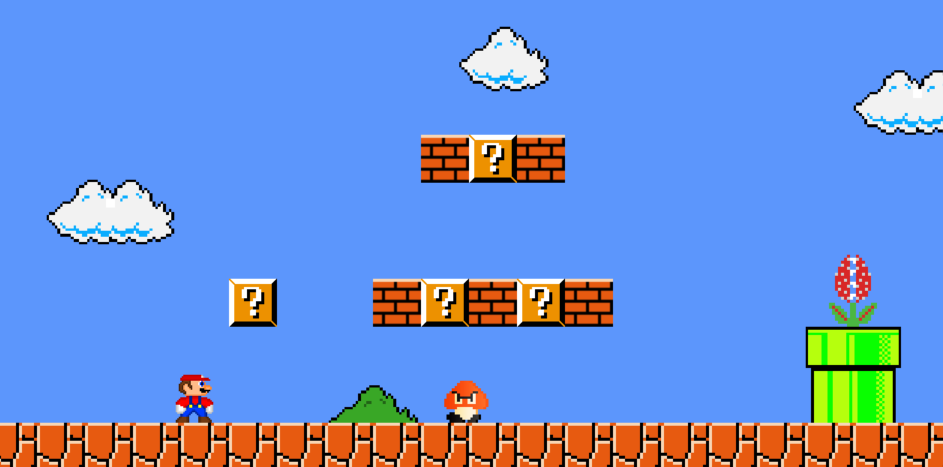
\includegraphics[scale=0.4]{img/game.png}
    \caption{Grafika koncepcyjna przedstawiająca grę.}
\end{figure}

\section*{Edytor poziomów}

Do gry dołączony będzie edytor poziomów, który pozwala na umieszczanie 
elementów na mapie za pomocą myszy i zapisywanie poziomu do pliku w odpowiednim 
formacie, który może zostać wczytany przez grę.

Edytor operuje na kilku warstwach (np. tło, bloki z których zbudowane są 
platformy, obiekty poruszające się), pomiędzy którymi można się przełączać.

\begin{figure}
    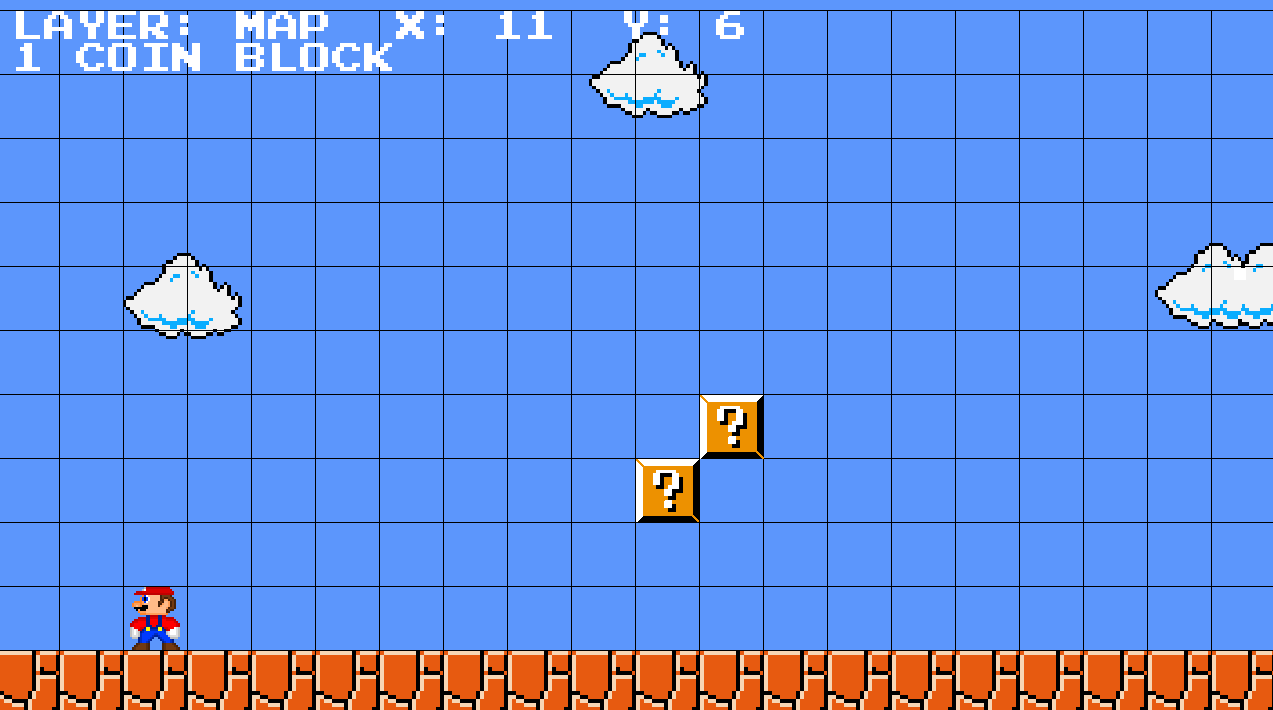
\includegraphics[scale=0.3]{img/editor.png}
    \caption{Grafika koncepcyjna przedstawiająca edytor poziomów.}
\end{figure}

\section*{Najważniejsze używane biblioteki}

\begin{itemize} 
    \item{\texttt{sdl2} -- do tworzenia okna, wyświetlania w nim grafiki i 
    obsługi klawiatury i myszy}
    \item{\texttt{serde\_json} -- do parsowania plików w formacie \texttt{json} 
    zawierających m.in. konfigurację gry}
    \item{\texttt{vector2d} -- do operacji na wektorach przy obliczeniach 
    związanych z fizyką}
\end{itemize}

\section*{Planowana organizacja kodu}

Stan gry reprezentowany będzie przez strukturę \texttt{GameState}, która 
przechowuje wszystkie informacje związane ze stanem programu (np. strukturę 
opisującą postać gracza, aktualny poziom, informację o tym, czy gracz jest w 
edytorze poziomów/menu/grze, aktualny stan klawiatury). W każdej klatce (czyli 
w założeniu 60 razy na sekundę) następuje aktualizacja tej struktury w oparciu 
o wydarzenia, których dostarcza biblioteka \texttt{sdl2} (np. naciśnięcia 
klawiszy) oraz dotychczasowego stanu gry. Po zaktualizowaniu stanu zostaje on w 
odpowiedni sposób wyświetlony na ekranie.
\newline

Kod gry jest dostępny na publicznym repozytorium na \href{https://github.com/JakubGrobelny/mario-clone}{githubie}.

\end{document}
